%%%%%%%%%%%%%%%%%%%%%%%%%%%%%%%%%%%%%%%%%%%%%%%%%%%%%%%%%%%%%%%%%%%%%%%%%%%%%%%%
%%
%% Uppsala Beamer theme example by Frédéric Haziza <daz@it.uu.se>
%%
%% Describing beamerthemeUppsala version 2008/05/15
%%
%% If you have more than three sections or more than three subsections in at least
%% one section, you might want to use the [hideallsubsections] or
%% [hideothersubsections] switch.  In this case, only the current (sub-) section is
%% displayed in the sidebar and not the full overview.
%%
%% Options are:
%% ===========
%% * hideallsubsections, hideothersubsections
%% * nonumbers,totalnumber
%% * withnav, mylogo
%% * grey
%% * noprogressbar
%%
%% For the sidebar layout:
%% * subsectionsattop, sectionpathattop
%% 
%% Removed
%% =======
%% * sidebarshades
%%
%% Tip
%% ===
%% latex this file to see the theme in action
%%
%%%%%%%%%%%%%%%%%%%%%%%%%%%%%%%%%%%%%%%%%%%%%%%%%%%%%%%%%%%%%%%%%%%%%%%%%%%%%%%%

\documentclass{beamer}
%\documentclass[handout]{beamer}
%\documentclass[notes]{beamer}
%\documentclass[trans]{beamer}

\usetheme[hideothersubsections,withnav]{BioExcel}

\usepackage{hyperref}
\usepackage{pgf}
\usepackage{tikz}
\usepgflibrary{arrows}
\usepgflibrary{shapes}
\usetikzlibrary{%
  arrows,%
  calc,%
  fit,%
  patterns,%
  plotmarks,%
  shapes.geometric,%
  shapes.misc,%
  shapes.symbols,%
  shapes.arrows,%
  shapes.callouts,%
  shapes.multipart,%
  shapes.gates.logic.US,%
  shapes.gates.logic.IEC,%
  er,%
  automata,%
  backgrounds,%
  chains,%
  topaths,%
  trees,%
  petri,%
  mindmap,%
  matrix,%
  calendar,%
  folding,%
  fadings,%
  through,%
  positioning,%
  scopes,%
  decorations.fractals,%
  decorations.shapes,%
  decorations.text,%
  decorations.pathmorphing,%
  decorations.pathreplacing,%
  decorations.footprints,%
  decorations.markings,%
  shadows}

\usepackage[english]{babel} % or whatever
\usepackage[utf8]{inputenc} % or whatever
\usepackage{graphicx}
%%\usepackage{caption}
\usepackage[labelformat=empty]{caption}
\usepackage[font=footnotesize]{subcaption}
\setbeamerfont{caption}{size=\tiny}
\setbeamerfont{frametitle}{size=\small}
\usepackage{mathptmx}
\usepackage{helvet}
\usepackage{overcite}
\usepackage{fixltx2e}
\usepackage{multirow}
\usepackage{tabularx}
%\usepackage{courier}

\usepackage[T1]{fontenc}
\usepackage[num,UKenglish]{isodate}
% Or whatever. Note that the encoding and the font should match. If T1
% does not look nice, try deleting the line with the fontenc.

%% -----------------------------------------------------------
%% MISC. INFORMATION
%% -----------------------------------------------------------
\numberwithin{table}{section}
\numberwithin{figure}{section}
\numberwithin{equation}{section}

\title{\emph{Umbrella sampling in GROMACS}}
\subtitle{BioExcel Summer School 2018}

\author[Paul Bauer]%| \emph{paul.bauer@icm.uu.se}] % appears in the footline
{Paul Bauer <\texttt{paul.bauer@scilifelab.se}>}

\institute[SciLifeLab, KTH] % appears in the footline
{
  SciLifeLab\\
  KTH
}

\date[\footnotesize{\today}] % appears in the bottom of the sidebar
{\today}

%% \logo{...}

%% This is only inserted into the PDF information catalog. Can be left out.
\subject{BioExcel Summer School 2018}

%% -----------------------------------------------------------
%% Extra ``local'' settings
%% -----------------------------------------------------------

% Comment out this, if you do not want the table of contents to pop up at
% the beginning of each (sub)section:
% \AtBeginSection[]
% {
%   \begin{frame}<beamer> % with <beamer> => doesn't appear in handout mode
%     \frametitle{Outline} %% Put the title you want, or none!
%   %\tableofcontents[currentsection,currentsubsection]
%     \tableofcontents[currentsection,hideallsubsections]
%   \end{frame}
% }

%% Unfolds piecewise element with shading.
%% Text appears, shaded, and the audience knows that somehting is coming
%% Note: if you set the number too high, the audience will try to read the 
%% text that now shows up more, and will be disturbed.
%% ``dynamic'' makes elements show gradually more and more.
\setbeamercovered{transparent=5}
%% \setbeamercovered{dynamic=5}

%% -----------------------------------------------------------

\renewcommand{\vec}[1]{\mathbf{#1}}

\begin{document}

\begin{frame}[plain] %% Gets the frame to fill up the page, no menu/sidebar/footline
  \titlepage
\end{frame}

\begin{frame}
    \frametitle{Outline}
    \tableofcontents[hideallsubsections]
\end{frame}


\section{Basics of Umbrella Sampling (US)}

\begin{frame}
\frametitle{Sampling problems in Molecular Dynamics}
    \begin{figure}[htb]
        \centering
        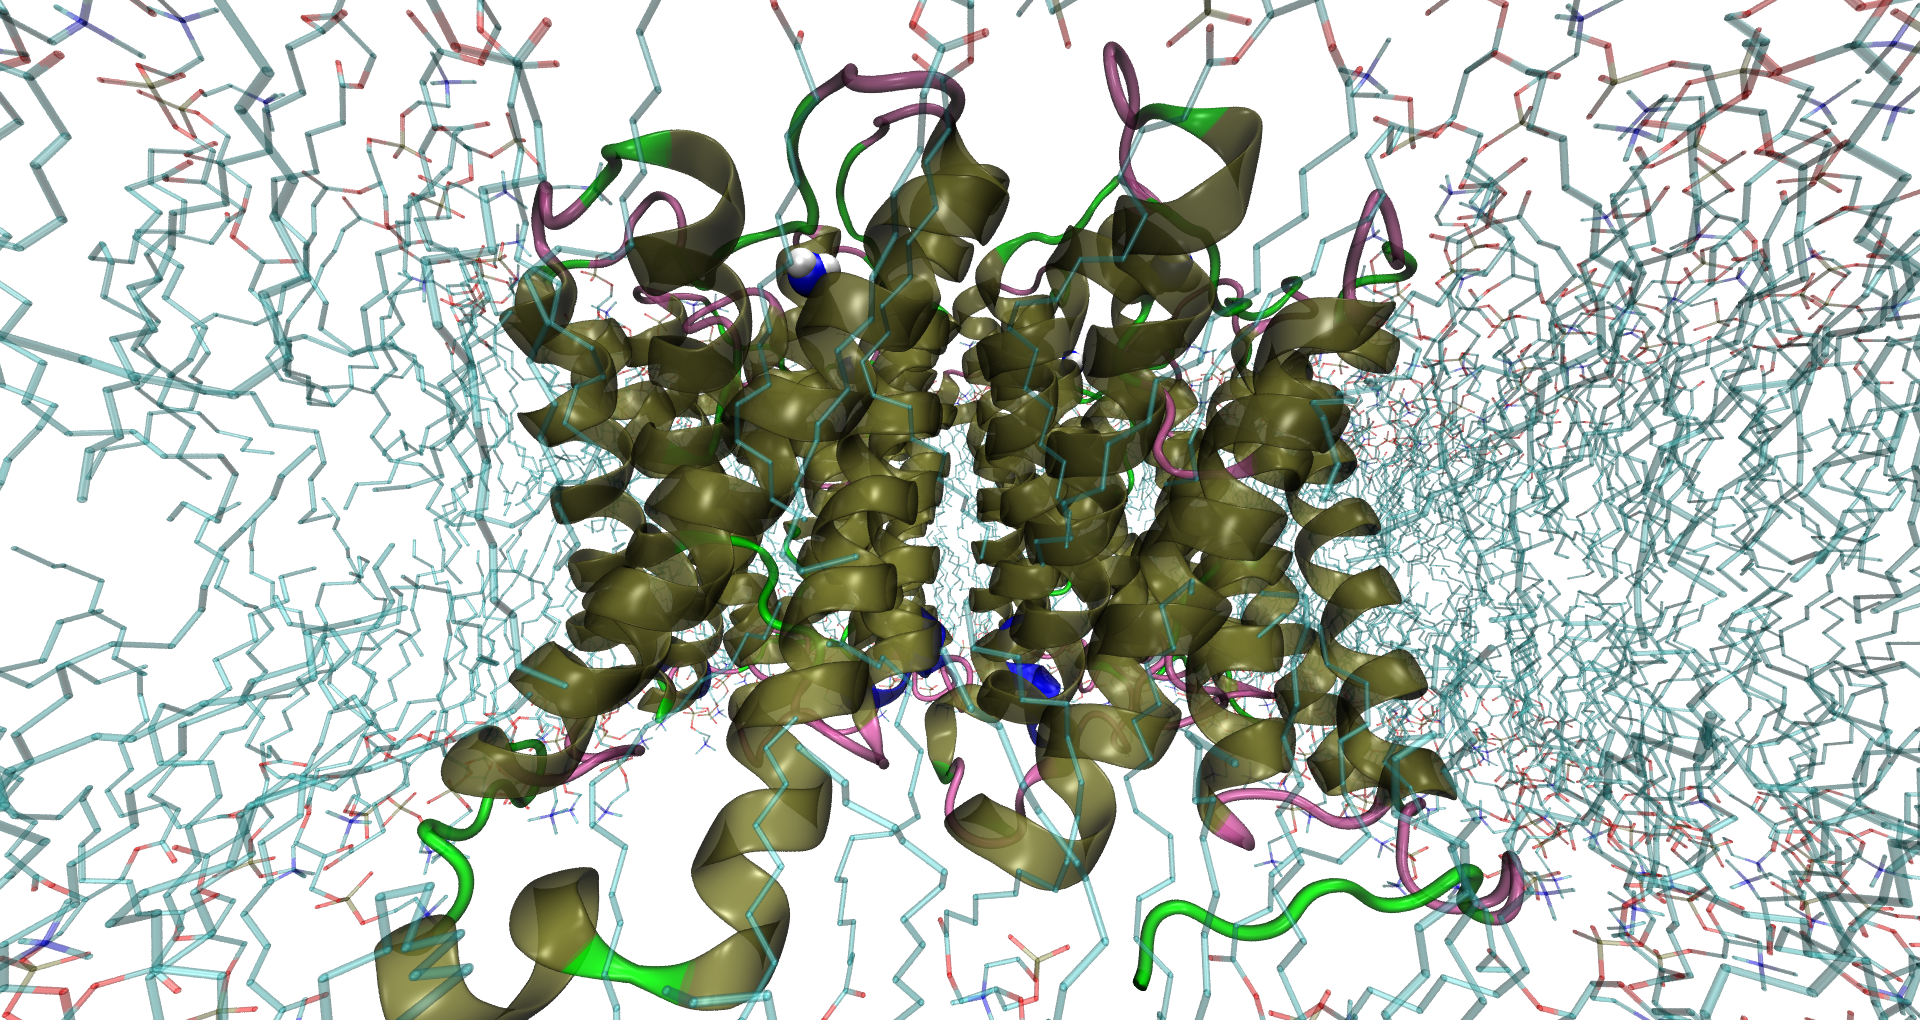
\includegraphics[keepaspectratio=true, width=0.8\textwidth]{figures/system.png}
        \caption{Example problem being studied by MD: Transport of a solute through a membrane channel.}
    \end{figure}
\end{frame}

\begin{frame}
\frametitle{Covering of complete phase space is unrealistic}
    \begin{itemize}
        \item{Systems explore phase space according to boundary conditions given by the ensemble}
        \item{Larger differences in energy between states make crossing less likely}
        \item{Interesting changes often involve large changes in free energy and large free energy barriers}
        \item{System needs to be forced to either cross barriers or ignore them}
    \end{itemize}
\end{frame}

\begin{frame}
\frametitle{Biasing potentials help crossing of free energy barriers}
        {Basic math behind use of Umbrella Sampling}
        {
                \begin{eqnarray*}
                    U_{\text{window}}\left( \vec{r} \right) &=& U\left( \vec{r}\right) + W\left( \vec{r}_{\text{rest}} \right) \\
                    W\left( \vec{r}_{\text{rest}} \right) &=& k\left( \vec{r} - \vec{r}_{ref} \right)^2
                \end{eqnarray*}
        }
        {System is moved through several windows with different references coordinates.}
\end{frame}

\begin{frame}
\frametitle{Example visualization of US windows}
    \begin{figure}[htb]
        \centering
        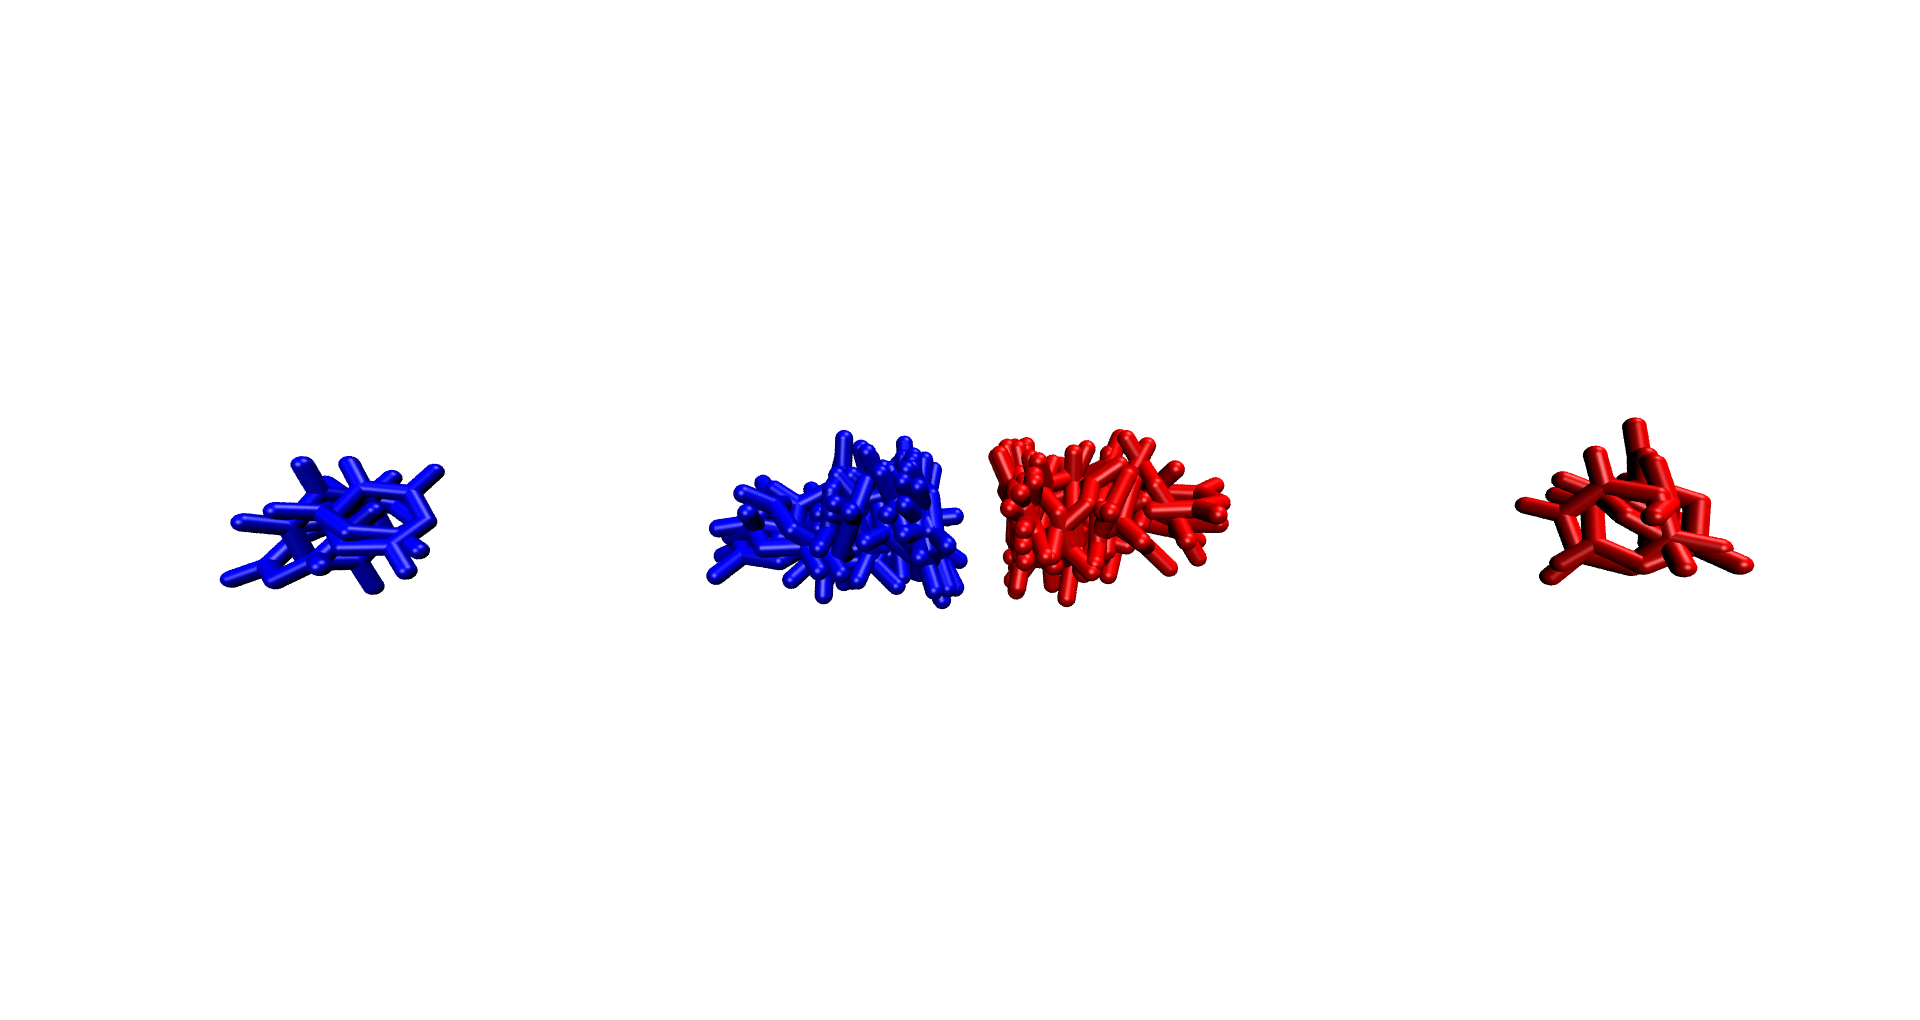
\includegraphics[keepaspectratio=true, width=0.8\textwidth]{figures/pyrimidine-us.png}
        \caption{Moving two pyrimidine molecules through different US windows.}
    \end{figure}
\end{frame}

\begin{frame}
\frametitle{Ways to define US window coordinates}
    \begin{figure}[htb]
        \centering
        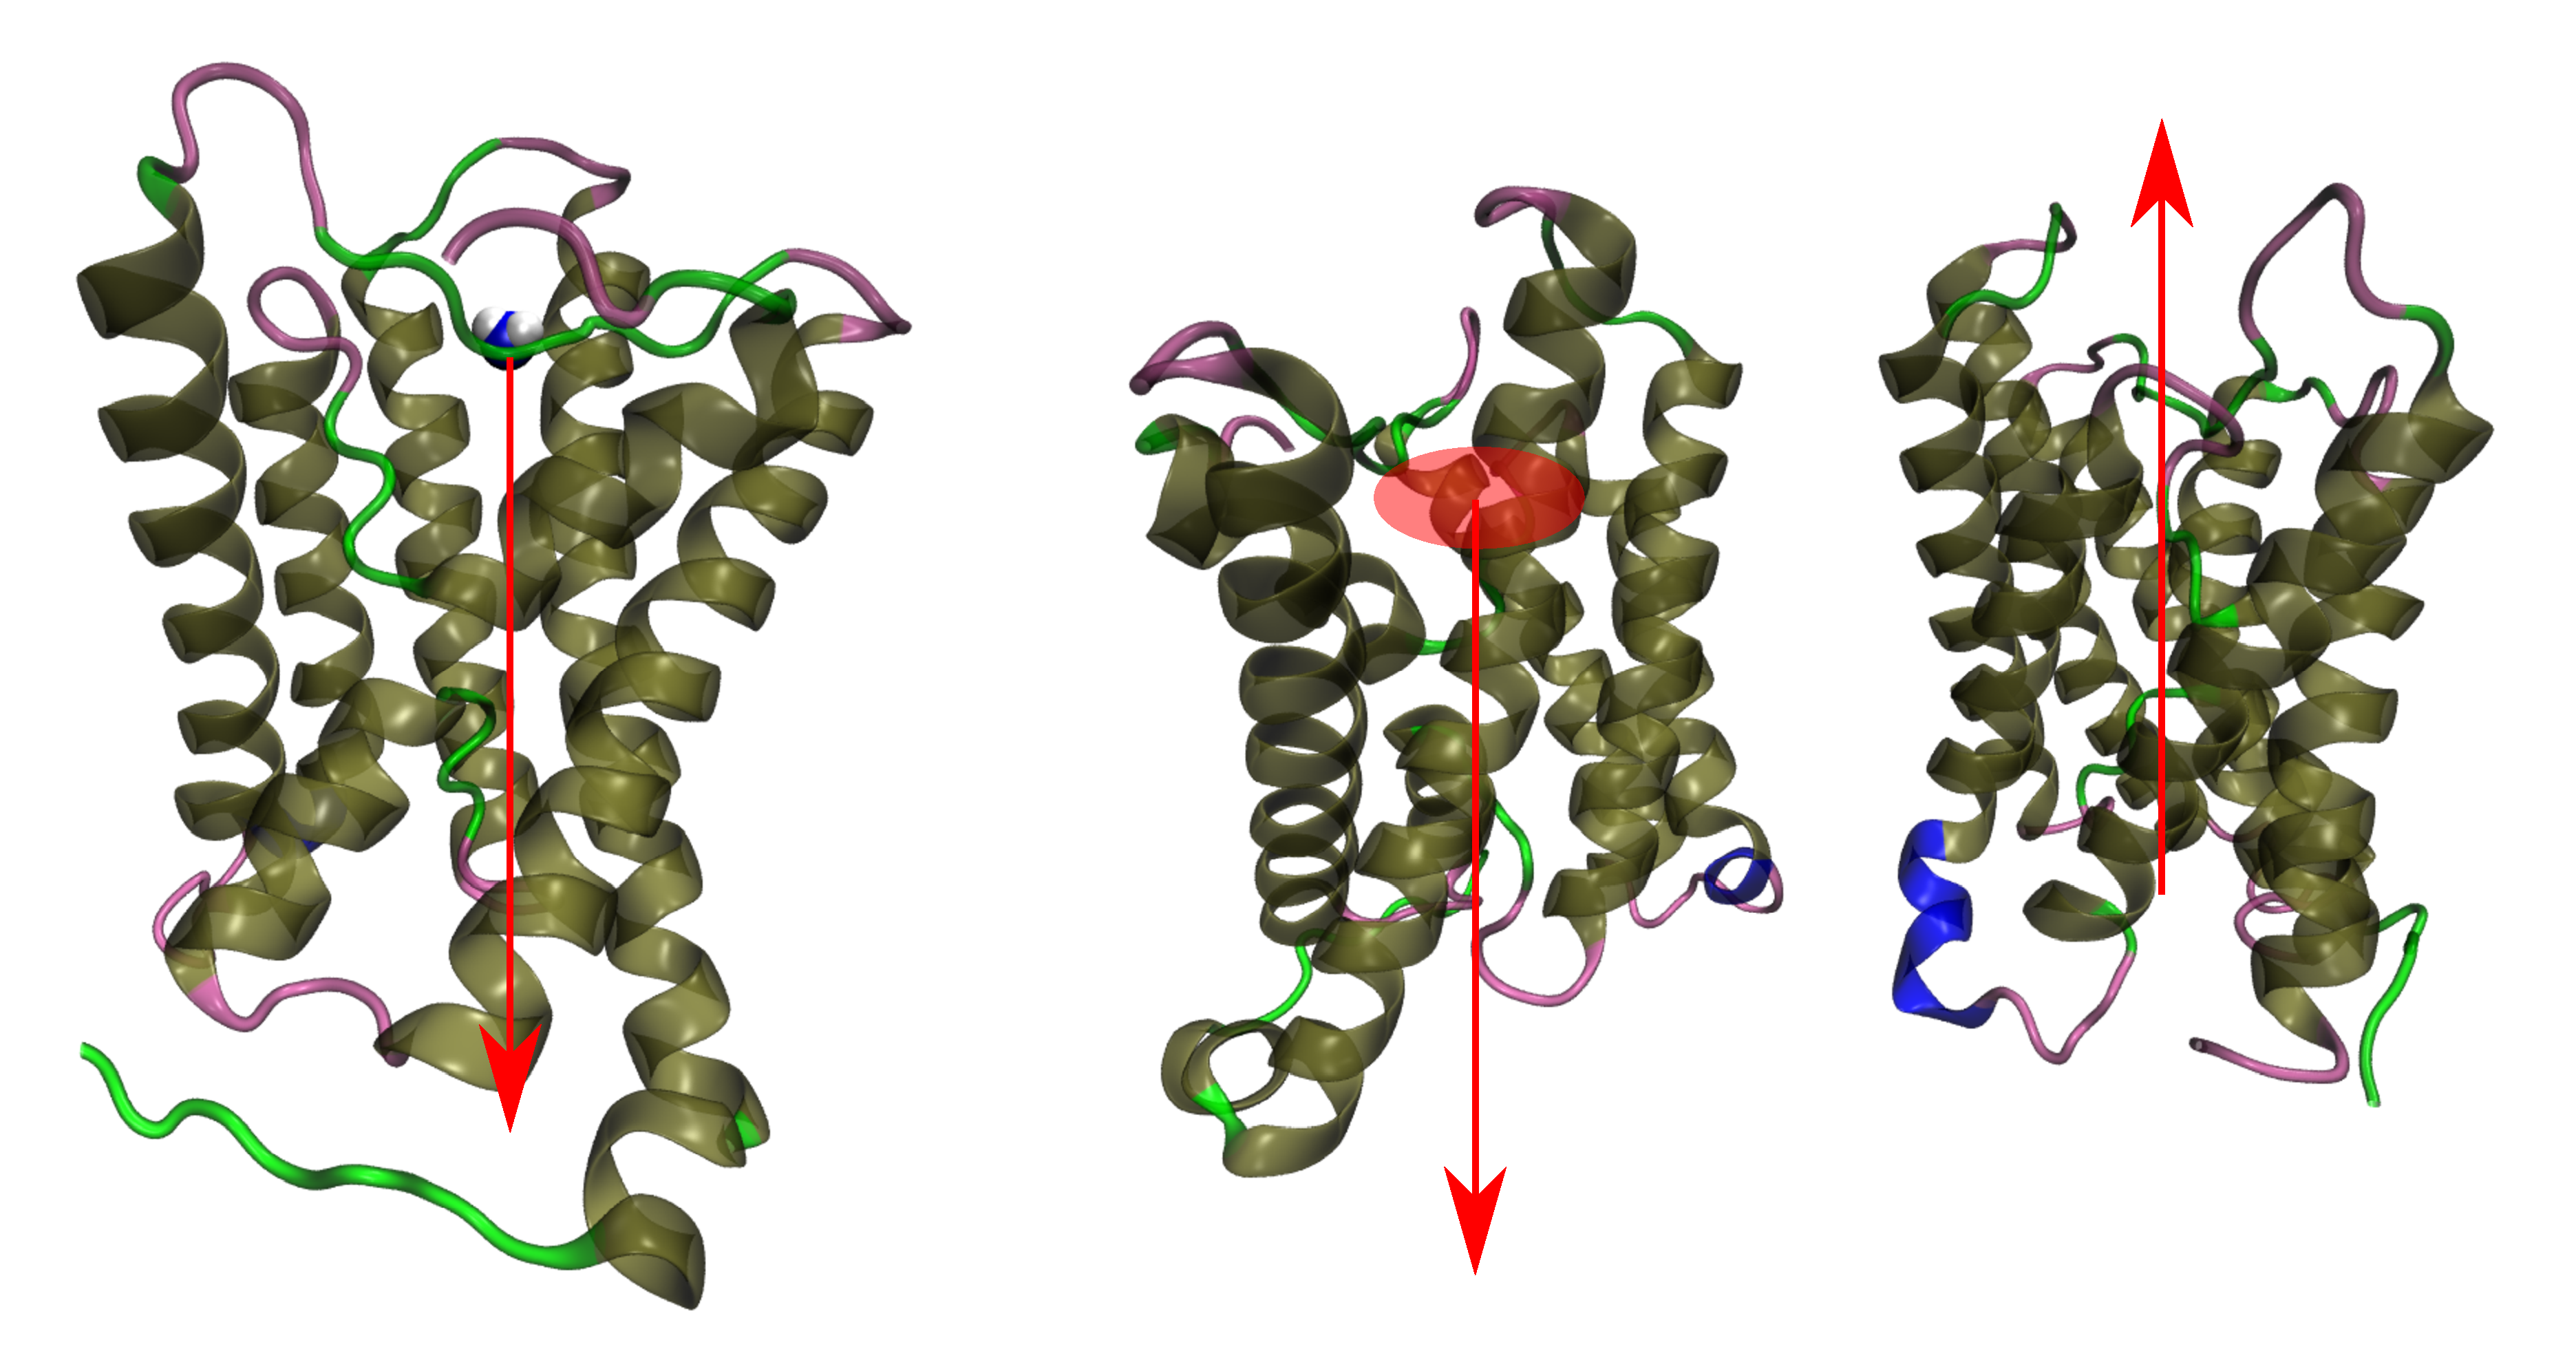
\includegraphics[keepaspectratio=true, width=0.8\textwidth]{figures/us-coord-define.pdf}
        \caption{Different ways to define US window coordinates.}
    \end{figure}
\end{frame}

\begin{frame}
\frametitle{Minimum requirements for converging simulation}
    \begin{itemize}
        \item{Each window needs to represent physical configuration}
        \item{Windows need to have sufficient sampling overlap}
        \item{No large changes between configurations that can't be sampled}
    \end{itemize}
\end{frame}

\begin{frame}
\frametitle{How to generate initial configurations?}
    \begin{itemize}
        \item{Manual placement of initial configurations}
        \item{Molecular dynamics with constant potential}
        \item{Simulation with restraints}
        \item{QM calculations}
    \end{itemize}
%%    \begin{figure}[htb]
%%        \centering
%%        \includegraphics[keepaspectratio=true, width=0.8\textwidth]{figures/us-generate-conf.pdf}
%%        \caption{How to generate different initial configurations for US}
%%    \end{figure}
\end{frame}

\begin{frame}
\frametitle{Some application examples}
    \begin{itemize}
        \item{Calculation of dimerization energies}
        \item{Clearly defined change within simulated structure}
        \item{QM/MM for chemical reactions in enzyme systems}
        \item{What can you think of?}
    \end{itemize}
\end{frame}

\section{Umbrella sampling in GROMACS}

\begin{frame}
\frametitle{US basics and requirements}
    \begin{itemize}
        \item{All here based on reasonable recent version of GROMACS, tried on v2018}
        \item{Examples and later tutorials based on \url{https://barnett.science/tutorials/5_umbrella/}}
        \item{Need to understand pull code, index groups, (partially) WHAM}
        \item{Topology setup and definition not covered}
    \end{itemize}
\end{frame}

\begin{frame}
\frametitle{Introduction to index groups}
    \begin{figure}[htb]
        \centering
        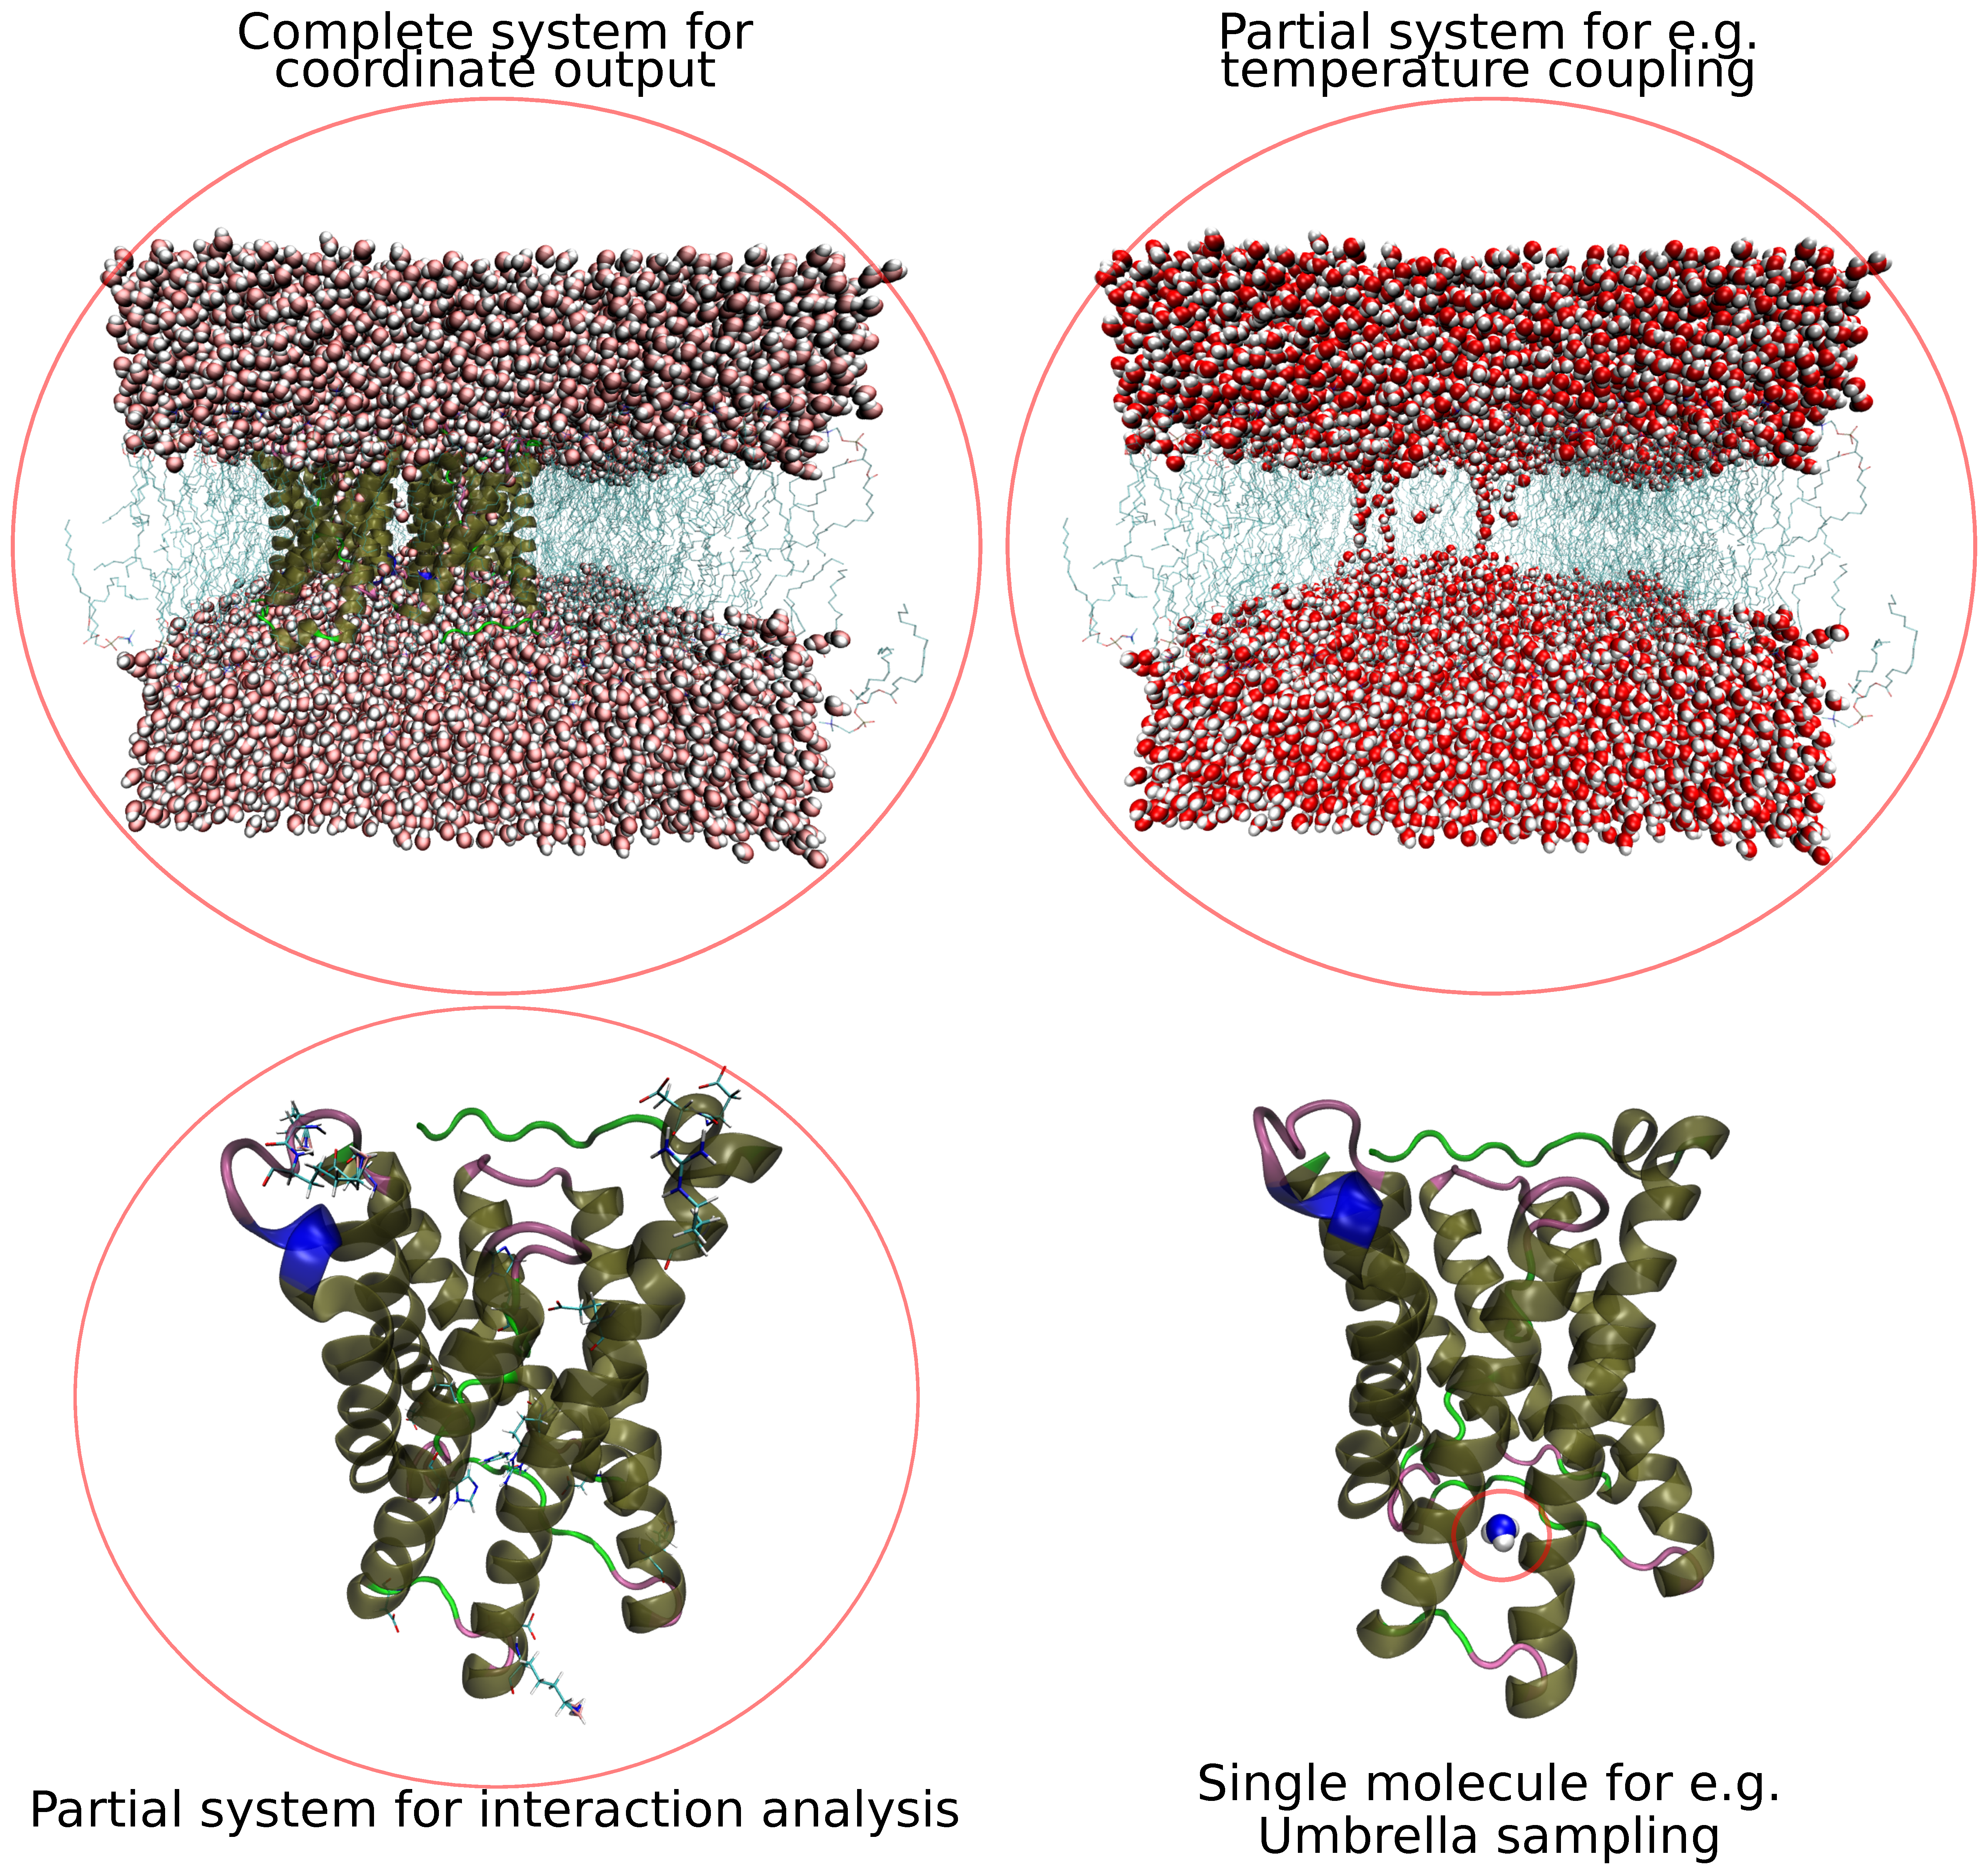
\includegraphics[keepaspectratio=true, width=0.8\textwidth]{figures/index-groups.pdf}
        \caption{Examples for index groups}
    \end{figure}
\end{frame}

\begin{frame}
\frametitle{Index group basics}
    \begin{itemize}
        \item{List of atoms being grouped together according to some requirement}
        \item{Used to specify important parts of simulation for running/analysis/data processing}
        \item{Defaults generate by all GROMACS tools internally}
        \item{User defined groups available through either gmx make\_ndx or gmx select}
    \end{itemize}
\end{frame}

\begin{frame}
\frametitle{How to generate index files with make\_ndx}
    \begin{figure}[htb]
        \centering
        
\includegraphics[keepaspectratio=true, width=0.8\textwidth]{figures/demo.pdf}
        \caption{Demo time!}
    \end{figure}
\end{frame}

\begin{frame}
\frametitle{Setting up the simulation}
    \begin{itemize}
        \item{Define groups that should be restrainted by US windows}
        \item{Define coordinates to be used for restraint}
        \item{Set window spacing or generate initial configurations}
        \item{Set US window restraint force constant}
    \end{itemize}
\end{frame}

\begin{frame}
\frametitle{Different kinds of coordinates and geometries}
    \begin{itemize}
        \item{Linear distance}
        \item{Directional or based on reference}
        \item{Cylinder pulling}
    \end{itemize}
    \begin{figure}[htb]
        \centering
        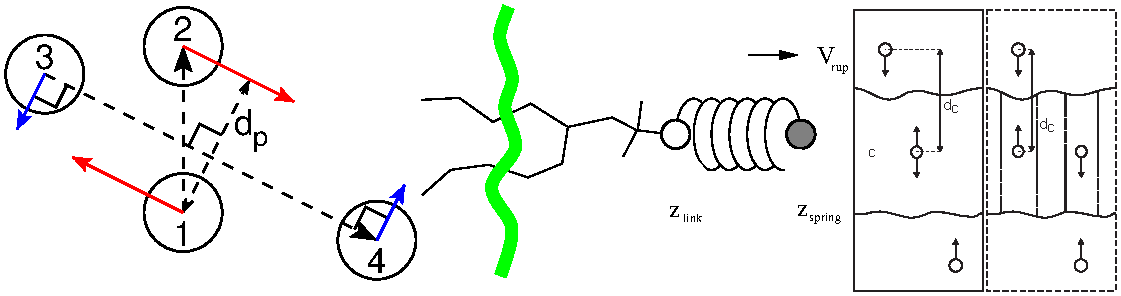
\includegraphics[keepaspectratio=true, width=0.8\textwidth]{figures/pull-coordinates.pdf}
        \caption{Examples for pull or US coordinates in GROMACS from reference manual}
    \end{figure}
\end{frame}

\section{Data analysis with gmx wham}

\begin{frame}
\frametitle{Basics of US histogram analysis}
    \begin{itemize}
        \item{All information here based on \url{http://doi.org/10.1002/jcc.540130812}}
        \item{Full disclosure: I'm not an expert in WHAM}
        \item{More intendet as opening point to look for further information}
    \end{itemize}
\end{frame}

\begin{frame}
\frametitle{Math behind WHAM}

    \begin{eqnarray*}
        P_{\{\lambda\}j,{\beta}_{j}} \left(\{V\}, \zeta \right) =&
        \frac{\sum_{k=1}^{R} N_{k}\left( \{V\}, \zeta\right) \exp{ \left(-{\beta}\sum_{j=0}^{L} {\lambda}_{j}V_{j} \right)}}{\sum_{m=1}^{R} n_{m} \exp{ \left( f_{m} -{\beta}_{m} \sum_{j=0}^{L} {\lambda}_{j,m} V_{j} \right)}} \\\\
        \exp{\left(-f_{i}\right)} =& \sum_{\{V\}, \zeta} P_{\{\lambda\}j,{\beta}_{j}} \left(\{V\}, \zeta \right) \\\\
        \exp{\left(-f_{i}\right)} =& 
        \sum_{k=1}^{R} \sum_{t=1}^{n_{k}} \frac{\exp{\left[ -{\beta}_{i} \sum_{j=0}^{L} {\lambda}_{j,i} V_{j,t}^{(k)}\right]}}{\sum_{m=1}^{R} n_{m} \exp{\left[ f_{m} -{\beta}_{m} \sum_{j=0}^{L} {\lambda}_{j,m} V_{j,t}^{k} \right]}}
    \end{eqnarray*}
\end{frame}

\begin{frame}
\frametitle{Analysing GROMACS US simulations}
    \begin{itemize}
        \item{Needs at least run input file and pullx or pullf file for each window}
        \item{Will by default calculate both individual histograms and PMF}
        \item{Able to also obtain autocorrelation times and error estimates}
    \end{itemize}
\end{frame}

\begin{frame}
\frametitle{Example analysis from simple US simulation}
    \begin{figure}[htb]
        \centering
        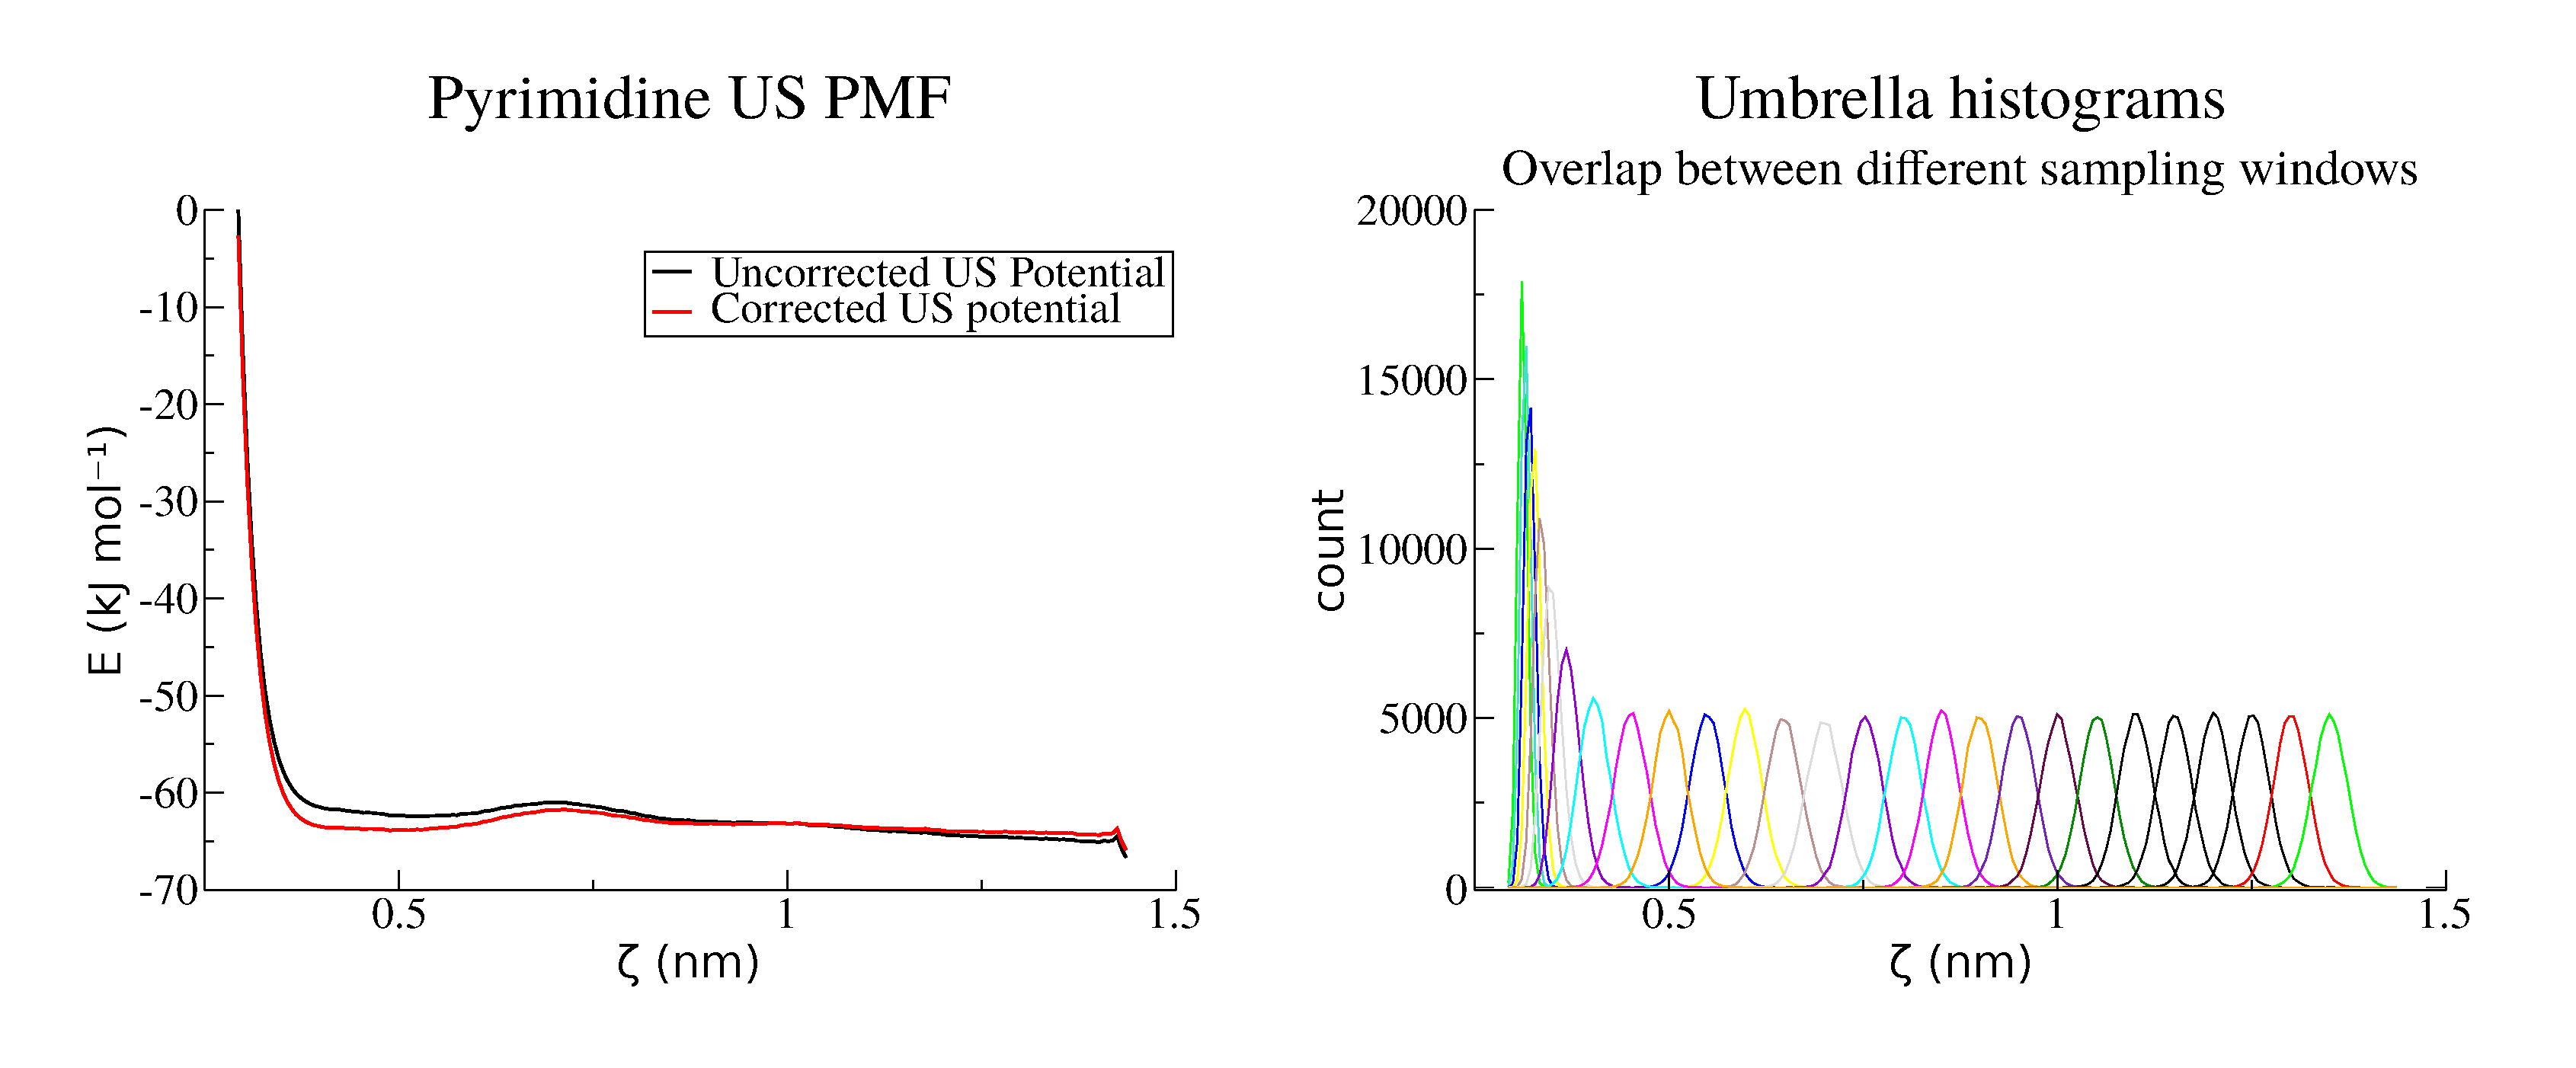
\includegraphics[keepaspectratio=true, width=\textwidth]{figures/histoprofile.pdf}
        \caption{Well coverged and overlapping US simulation}
    \end{figure}
\end{frame}

\begin{frame}
\frametitle{Common pitfalls}
    \begin{itemize}
        \item{Insufficient sampling overlap}
        \item{Bad choice of reaction coordinate}
        \item{Bad choice of restraint parameters}
        \item{Insufficient equilibration}
    \end{itemize}
\end{frame}

\begin{frame}
\frametitle{Thanks for your attention/patience}
    \begin{itemize}
        \item{Questions?}
        \item{Comments?}
        \item{Suggestions?}
    \end{itemize}
\end{frame}

\end{document}
